\section{WC 23/6/25}

\subsection*{Overview:}
This week marks the Launch of my EP Artifact: NeuroNote. 
\subsection*{Achievements, Thoughts and Ideas:}
Having pressed Publish on my website I have now launched NeuroNote to my waiting list of users (and anyone else who wishes to try it out). I am excited to see how they respond and what feedback they provide. Despite launching only this week I already have some incredible feedback, compliments and feature requests.

To launch I sent an email to my waitlist and messaged a number of peers on WhatsApp to share details:

\begin{figure}[H]
    \centering
    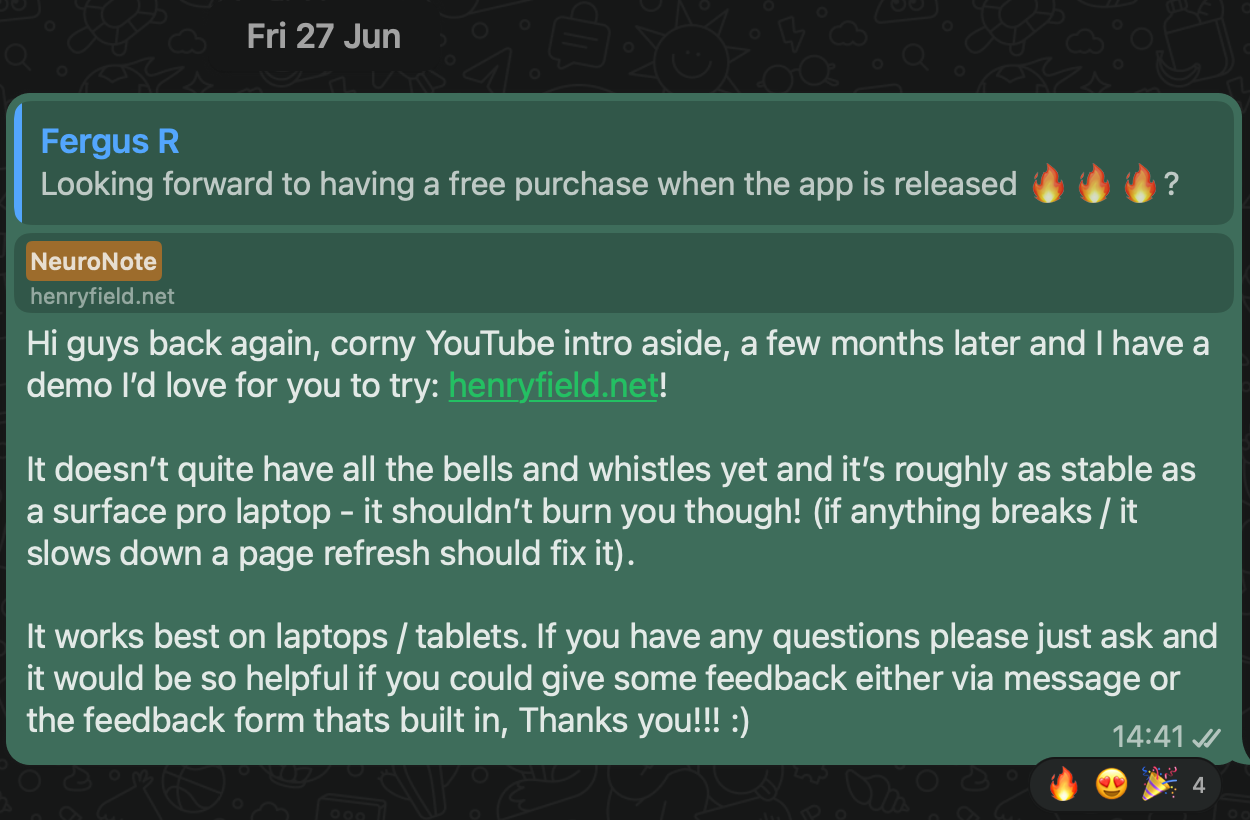
\includegraphics[width=0.6\textwidth]{Diary/34_WC_23-6-25/media/whatsappMessage.png}
    \caption{WhatsApp message to peers}
\end{figure}

To try and gauge reception between friends / peers of mine on the waitlist and external users I published the site to two domains. My personal website (henryfield.net, for peers / waitlist members) and the project specific domain (Neuronote.space, for external users). This way I can see how many people are visiting each site and how they are interacting with it. 

To help reach out to potential users outside my network I made a post to R/SideProject on Reddit as I identified this group to be inviting and welcoming to small upstart projects.

\begin{figure}[H]
    \centering
    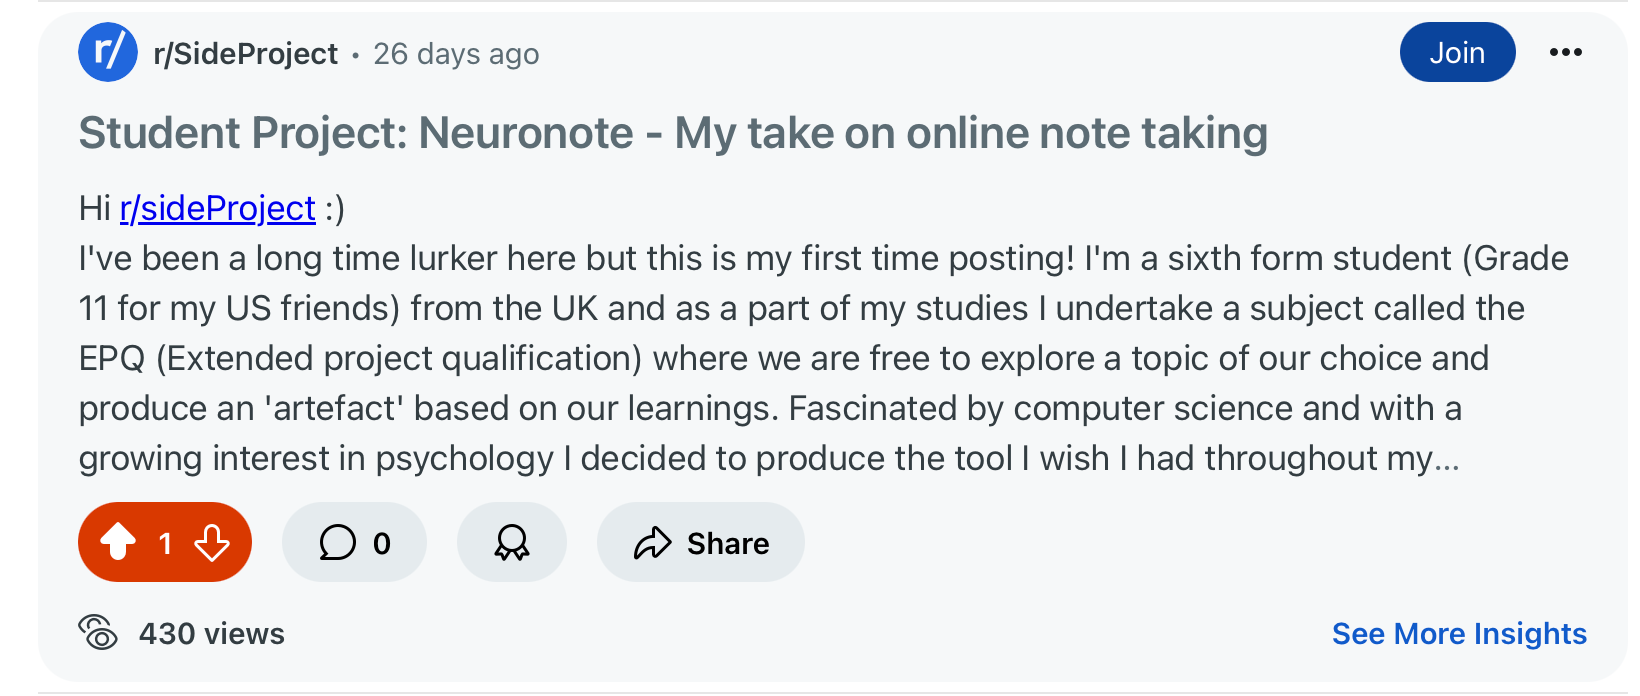
\includegraphics[width=0.6\textwidth]{Diary/34_WC_23-6-25/media/redditPost.png}
    \caption{Reddit post to promote my project}
\end{figure}

This post didn't perform quite as well as I had hoped however I did get over 400 views and a large number of signups (129 which weren't on my waitlist) which also helped me better gauge the success of my project. With a post capture rate of 32\% It seems that my project resonated well with students and young professionals who are looking to improve their productivity and focus. I hope to post to more online communities in the future to help promote my project and reach a wider audience.

\subsection*{What was challenging?}
With such an incredible reception to my project it did come along with some technical difficulties. One oversight I had made was a lack of password reset system. Having secured my system with a strong, fully encrypted password system I had not considered that users may forget their passwords and I could not easily provide them a new one. As a quick solution I requested users contact me via email or message if they needed help accessing their accounts and i=I would manually generate them a new (random) password that they could use to log in before changing it to something more memorable within the settings page. Whilst this wasn't ideal as some users may not change this temporary password it did seem to keep my users happy, and I processed 11 resets within the first 24 hours of launch. I see this high reset rate a positive sign as, whilst users may have initially used a random "keyboard bashing" password not expecting to use the site long term, they have since wanted to return and use my platform again and have taken the time to change their password to something more memorable.

One area where I potentially expected to face issues with was site stability / performance as I had not yet stress tested my site with a large number of real users. However, I am pleased to report that the site has been running smoothly and has not experienced any major issues or downtime. Thanks to Cloudflare CDN Caching over 85\% of requests are being served from the cache, which has helped to reduce the load on my server and improve performance. I have also been monitoring the site closely and have not seen any significant spikes in traffic or resource usage that would indicate a problem.

The only downtime faced was for 5 minutes on the 26th of June when a circuit breaker tripped within my home (thus also disactivating my redundant battery backup system, which was not as redundant as had first thought). Fortunately my mother was home and after some quick messages was able to resolve the issue and bring the server back online. 


\begin{figure}[H]
    \centering
    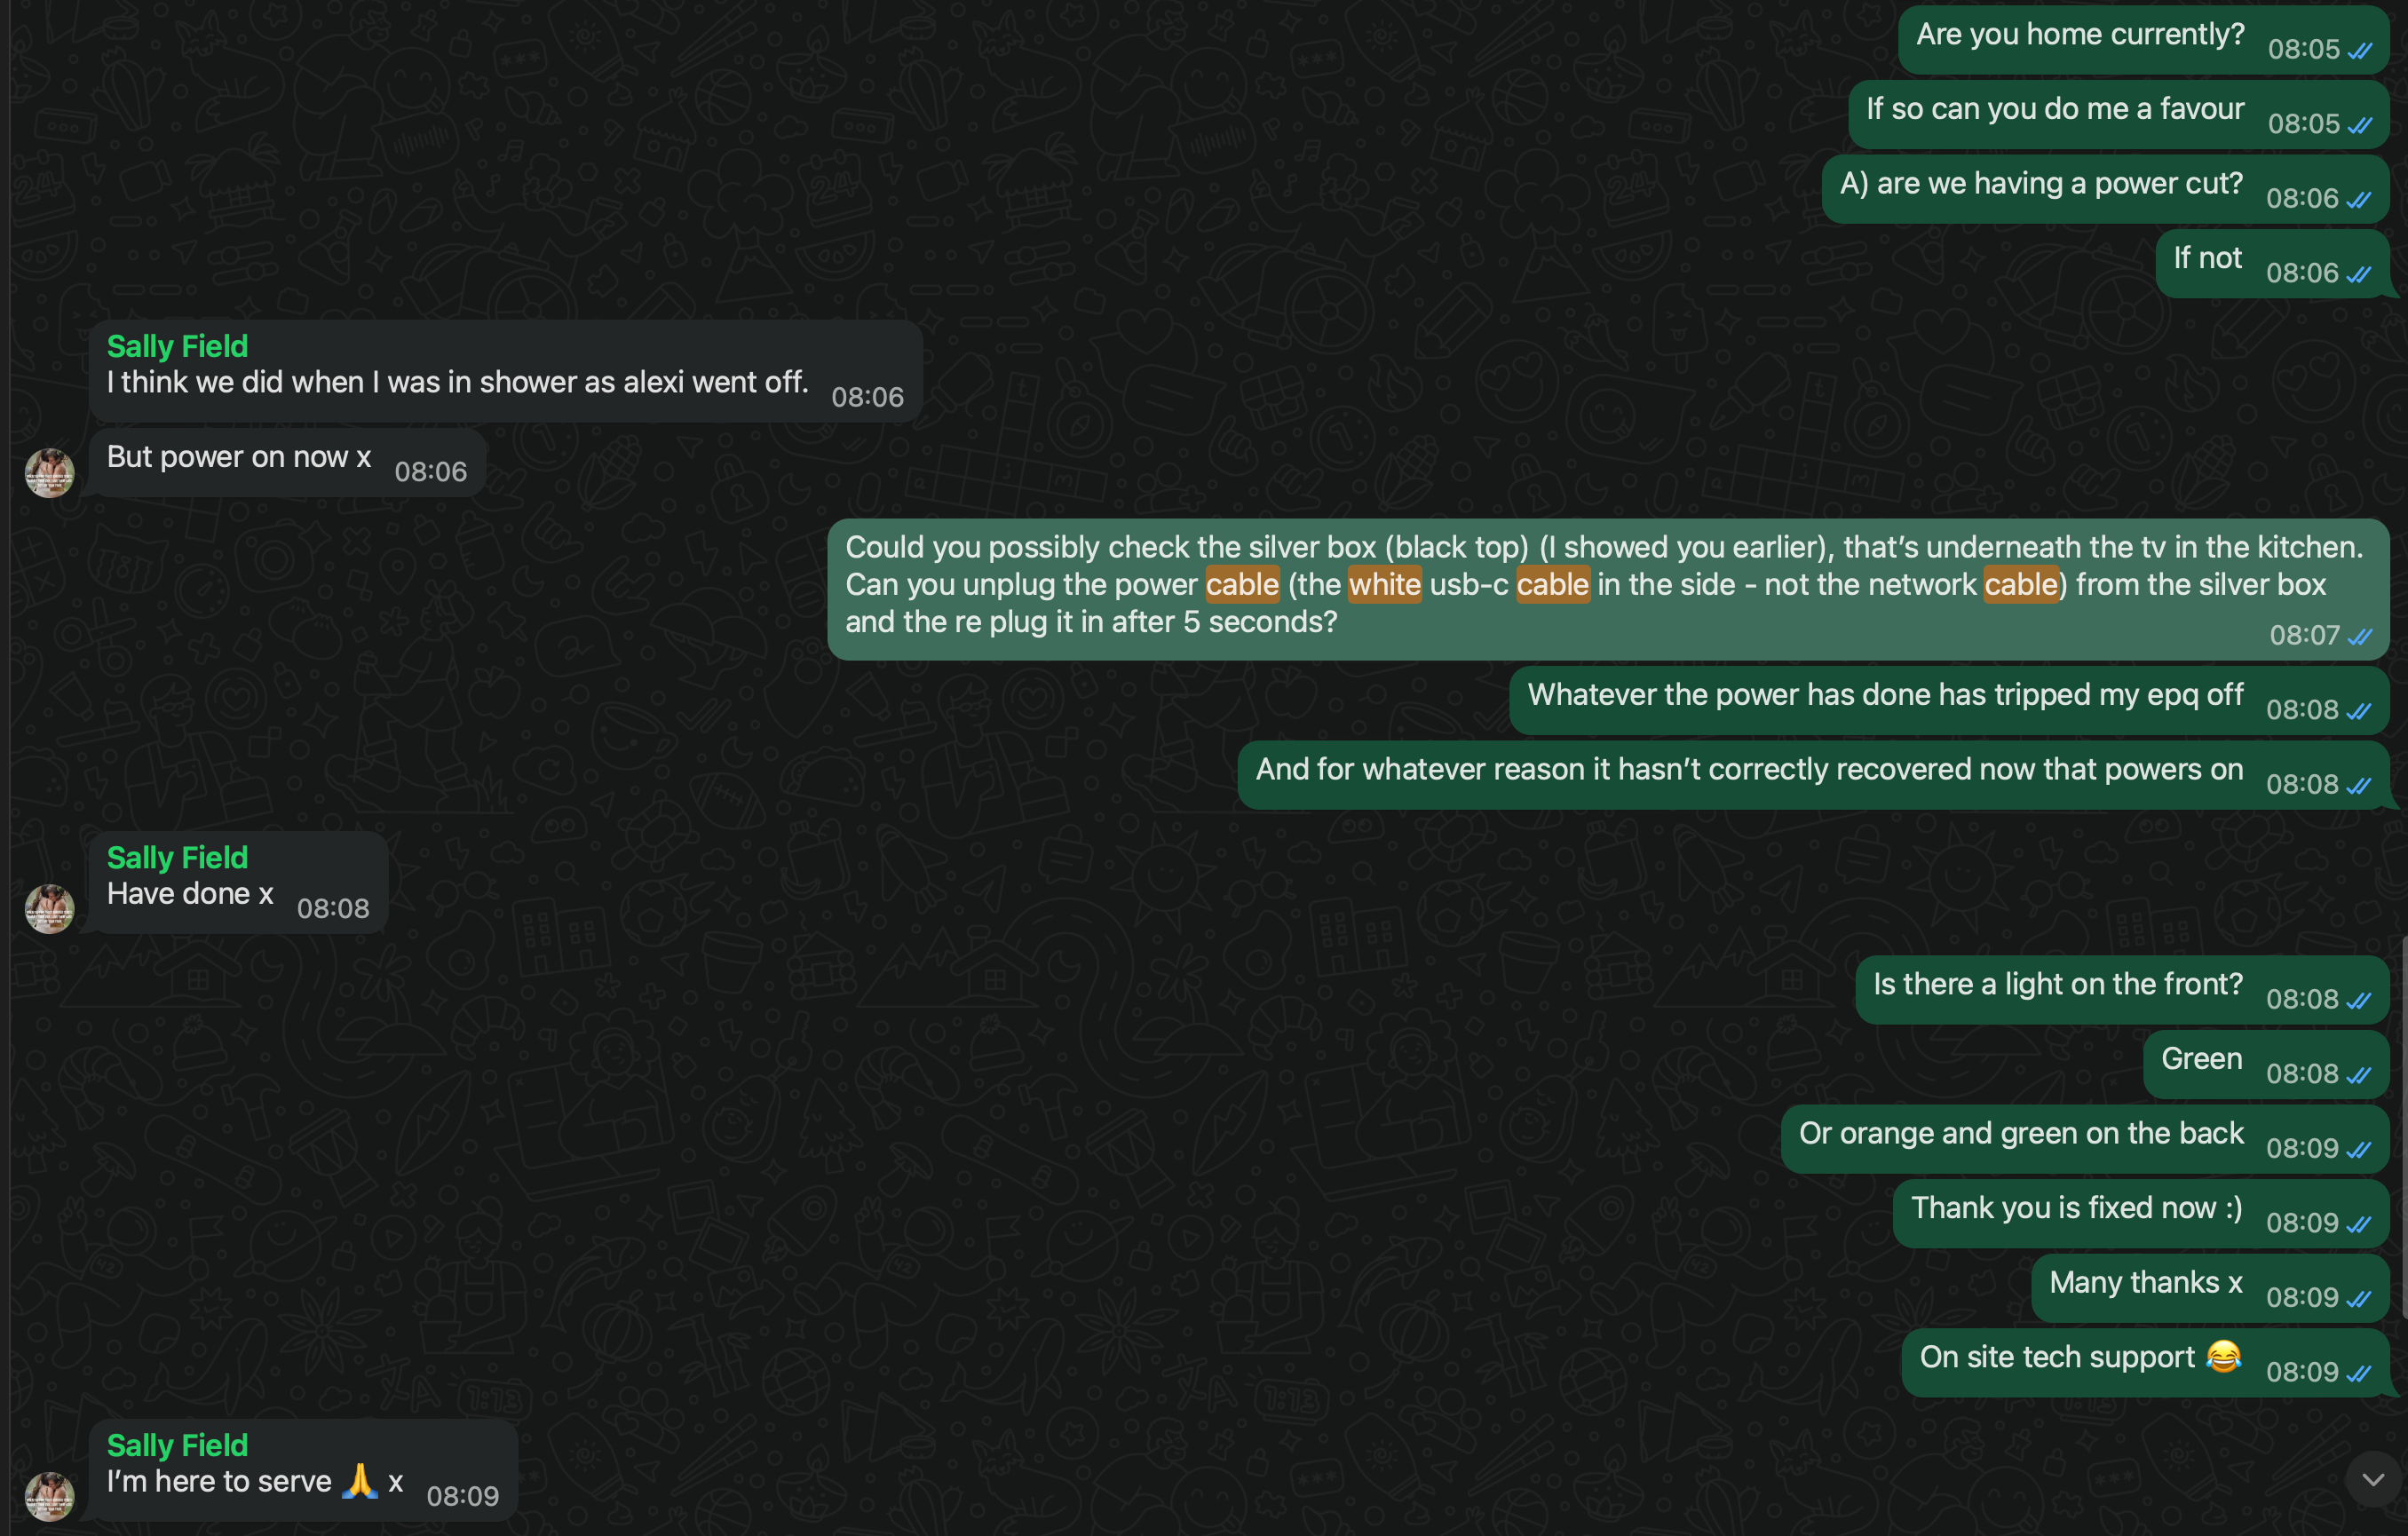
\includegraphics[width=0.6\textwidth]{Diary/34_WC_23-6-25/media/onSiteTechSupport.png}
    \caption{On site tech support from my mother :)}
\end{figure}

I first noticed the issue when I received an email from Uptime Robot that I had previously set-up to monitor my site. I am now very pleased I did so and this is a perfect showcase for why it is important to have monitoring in place for your website. Thankfully no users were affected by this downtime as it occurred during the early hours of the morning when traffic was low. Secondly I was pleased to have set up Tailscale as a VPN as I could remotely diagnose the issue whilst on a train in the countryside, truly available from anywhere

I was slightly confused at the time why the Raspberry Pi hadn't automatically restarted after the power was restored, however after some investigation I found that the Pi had fully shut down when the power cut out, not just 'died'. This behaviour is positive as it enabled the device to fully save all transactions resulting in no data loss. However, it did mean that the device was now waiting in standby for a user to physically press the power button, much like a laptop or personal computer. I have made sure to alter this configuration so that the Pi will always be running and accessible through SSH from anywhere, even after a power outage.

Whilst i appreciate outages such as these wouldn't be acceptable for a professional, to say that this system is running out of my kitchen cupboard and handling upwards of 200 users note-taking I think is very impressive. I am very pleased with the performance of my system and the fact that it has been able to handle the increased traffic without any major issues. 


I had a number of users report that they were unable to sign up to the site. After some investigation I found that this was due to a bug in my code that was preventing the signup form from working correctly. I have since fixed this issue and am now able to accept new users without any problems.